\section{Analysedokumentation}
    \subsection{Use Cases}
        \begin{enumerate}
          \item Start spillet
        \begin{itemize}
          \item Brugerne har mulighed for, at starte og slutte spillet. Evt. vha. vinduets knapper.
        \end{itemize}
         \item Kast terning
        \begin{itemize}
           \item Brugerne kan trykke på en knap for at kaste terningen.
        \end{itemize}
         \item Før spillets start, angiver brugeren antal spillere i et tekst-felt.
        \end{enumerate}
        
        
        \subsubsection{Use Case Diagram}
        
        \begin{figure}[H]
            \centering
            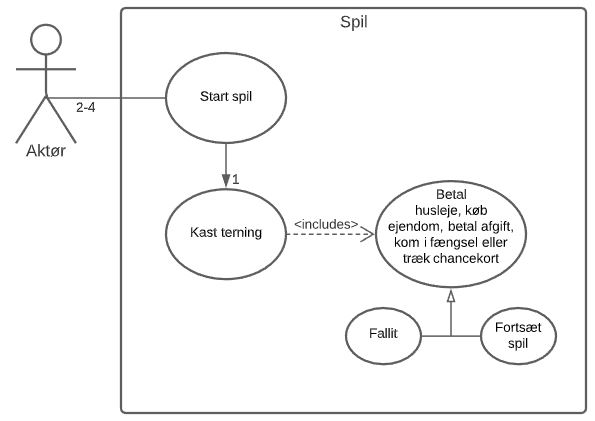
\includegraphics[width=10cm]{figures/usecase.jpg}
            \caption{Use Case Diagram}
            \emph{ Use Case Diagrammet viser hvordan en spiller interagerer med spillet}
        \end{figure}
        
        Når 2 til 4 spillere er blevet valgt og oprettet starter spiller. Aktørerne kan så kaste en terning som kører spillet. Alt efter hvilket felt de lander på, sker der forskellige ting, f.eks. at aktøren køber en grund. Programmet holder så øje med, om aktøren nu er gået fallit eller om spillet skal fortsætte til den næste aktør.

            

            
        \begin{table}[H]
        \centering
        \begin{tabular}{|p{0.3\linewidth} | p{0.6\linewidth}|} 
        \hline
        \textbf{Name}                         &\textbf{ Kaste terninger}  \\ 
        \hline
        Short description                     & Hver spiller har muligheden for at trykke på knappen og dermed kaste en terning\\ 
        \hline
        Precondition                          & For at en terning kan kastes, kræves det at spillet er i gang, og brugeren er klar til at starte sin tur\\ 
        \hline
        Postconditions                        & Terningerne viser et antal øjne og spilleren kan nu rykke til det ramte felt. Spillerens tur er nu slut.\\ 
        \hline
        Error situation                       & Spilleren var ikke klar til at kaste terningerne og dermed starte sin tur.\\ 
        \hline
        System state in the event of an error & Hvis en spiller ved fejl kaster terningerne, vil spillet stadig fortsætte uden mulighed for at vende tilbage.\\ 
        \hline
        Actors                                & Spiller 1 og 2.\\ 
        \hline
        Trigger                               & Knappen til kast af terning bliver trykket på af en af spillerne. \\ 
        \hline
        
        Standard process                      & 
        \begin{enumerate}
        \item Terningen får en tilfældig værdi mellem 1-6.
        \item Spilleren bliver rykket frem på spillepladen svarende til terningens værdi ud fra spillerens position.
        \item Der skal betales husleje svarende til feltets værdi.
        \end{enumerate}
        \\ 
        \hline
        
        Alternative processes                 &                  
        \begin{enumerate}
        \item Terninger viser en værdi mellem 1-6.
        \item Spilleren bliver rykket frem på spillepladen og lander på feltet \textit{fængsel}
        \item Spilleren er nu i fængsel og modtager ikke 2 {\rotatebox[origin=c]{180}{\textwon}} ved passering af start.
        \item Der skal betales 1 {\rotatebox[origin=c]{180}{\textwon}} for løsladelse af fængslet.
        \end{enumerate}
        \\
        \hline
        
        
        
        
        
        
        \end{tabular}
        \caption{Fully Dressed Use Case Diagram}
        \end{table}
        
        \clearpage
        
        \subsubsection{Fully Dressed Use Case}
        \textbf{Navn}\\
        Kaste terninger.\\
        
        \textbf{Scope}\\
        Kaste terninger benyttes af spillerene til at spille spillet. Denne Use Case benyttes hver tur.\\
        
        \textbf{Level}\\
        Viser antal øjne.\\
        
        \textbf{Primære aktører og interessenter} \\
        Spillerne er primære aktører. Der er ingen interessenter.\\
        
        \textbf{Forudsætning} \\
        Der skal være 2 spillere som starter spillet. Hver spiller skal være klar til at starte sin tur og dermed kaste terningerne. Hver spiller skal slå med terningen for at få point.\\
        
        \textbf{Succeskriterier} 
        \begin{itemize}
            \item Spilleren kaster terningen og lander på et felt.
            \item Spilleren reagerer til feltet ved enten at købe ejendommen, betale huslejen eller betale afgiften. 
            \item Turen går videre til næste spiller, som gør det samme. 
        \end{itemize}
        
        \bigskip
        
        \textbf{Succes Scenarie (Main Flow)}
        \begin{itemize}
            \item Spilleren kaster en terning.
            \item Spilleren ser hvilket felt han/hun er landet på.
            \item Spilleren betaler husleje, afgift eller køber ejendom
            \item Turen går videre til den næste spiller
        \end{itemize}
        
        %systemsekvensdiagram
        \begin{figure}[H]
            \centering
            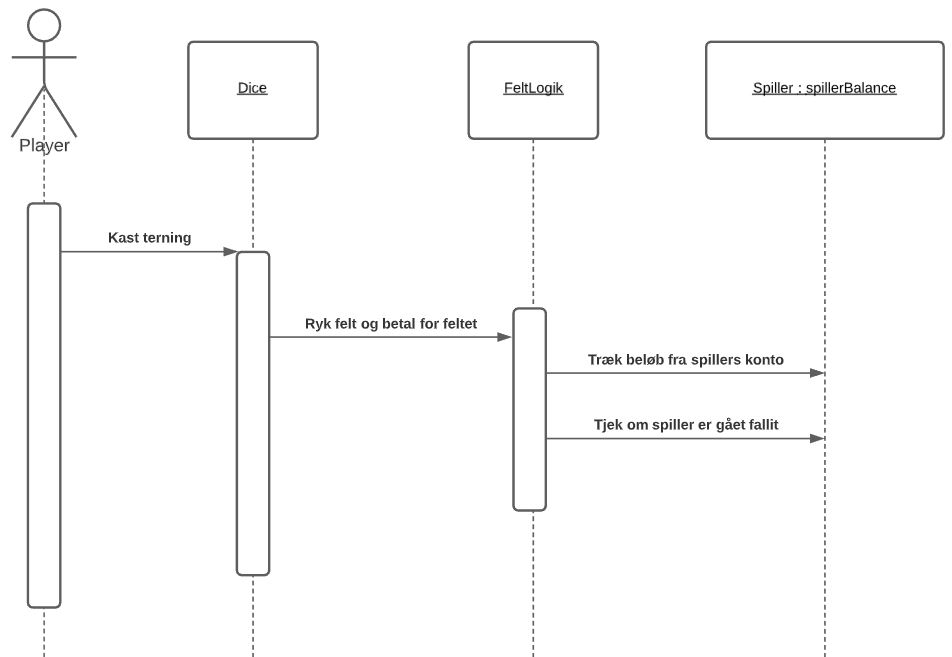
\includegraphics[width=14cm]{figures/systemSekvensDiagram.JPG}
            \caption{Systemsekvensdiagram}
            \emph{Systemsekvensdiagrammet viser step for step, hvilke handlinger spillet foretager. Dette Systemsekvensdiagrammet er tilføjet her for at illustrere et typisk succes scenarie ved brug af fully dressed use cases.}
        \end{figure}
        
        \textbf{Specielle krav} 
        \begin{itemize}
            \item Spillet skal åbnes af en spiller på en computer.
            \item Hver bruger kan fidne ud af at bruge en computer med en mus og keyboard.
        \end{itemize}
        
        \textbf{Frekvens}
        \begin{itemize}
            \item Use cases finder sted hver gang en spiller tager sin tur. 
        \end{itemize}
        
        
    \subsection{Domænemodel}
        \begin{figure}[H]
            \centering
            \includegraphics[width=14cm]{figures/domæneModel.JPG}
            \caption{Domæne model}
            \emph{Domænemodellen viser hvordan spillet fungerer. Det ses at én spiller kaster én terning, og rykker 1-6 felter frem. 4 felter på pladen med 24 udløser et chancekort.}
        \end{figure}
    \subsection{Systemsekvensdiagram}
        \begin{figure}[H]
            \centering
            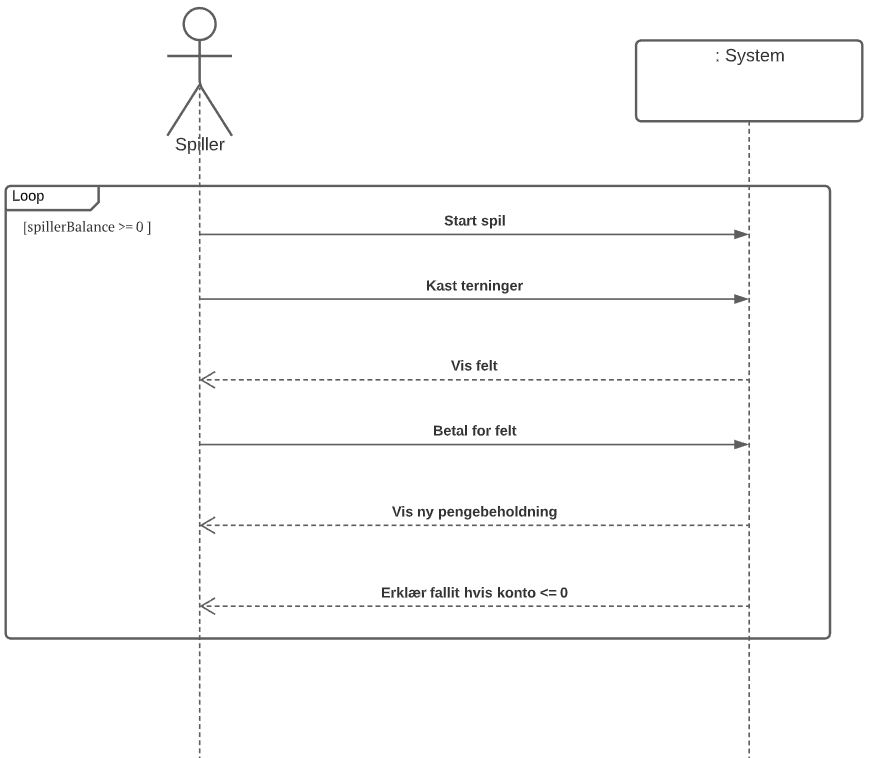
\includegraphics[width=14cm]{figures/overordnetSystemSekvensDiagram.JPG}
            \caption{Systemsekvensdiagram}
        \end{figure}

Systemsekvensdiagram viser hvordan en aktør interagerer med systemet som helhed. Har visualisere diagrammet, en aktørs muligheder når spillet spilles og dermed vises de metoder der tages i brug, når aktøren skal benytte spillet. Derudover viser diagrammet også, de handlinger som \textit{Systemet} selv foretager, når aktøren udfører en specifik handling. F.eks. når aktøren \textit{kaster terninger}, registrere systemet det og herefter udfører handlingen \textit{vis felt.}  
        

        
    
    
    
